%This is free and unencumbered software released into the public domain.
%
%Anyone is free to copy, modify, publish, use, compile, sell, or
%distribute this software, either in source code form or as a compiled
%binary, for any purpose, commercial or non-commercial, and by any
%means.
%
%In jurisdictions that recognize copyright laws, the author or authors
%of this software dedicate any and all copyright interest in the
%software to the public domain. We make this dedication for the benefit
%of the public at large and to the detriment of our heirs and
%successors. We intend this dedication to be an overt act of
%relinquishment in perpetuity of all present and future rights to this
%software under copyright law.
%
%THE SOFTWARE IS PROVIDED "AS IS", WITHOUT WARRANTY OF ANY KIND,
%EXPRESS OR IMPLIED, INCLUDING BUT NOT LIMITED TO THE WARRANTIES OF
%MERCHANTABILITY, FITNESS FOR A PARTICULAR PURPOSE AND NONINFRINGEMENT.
%IN NO EVENT SHALL THE AUTHORS BE LIABLE FOR ANY CLAIM, DAMAGES OR
%OTHER LIABILITY, WHETHER IN AN ACTION OF CONTRACT, TORT OR OTHERWISE,
%ARISING FROM, OUT OF OR IN CONNECTION WITH THE SOFTWARE OR THE USE OR
%OTHER DEALINGS IN THE SOFTWARE.
%
%For more information, please refer to <http://unlicense.org>


Dies ist ein dummy text um alle möglichen Formatierungen darzustellen um so 
Probleme zu finden.

\bigskip
Hier ein direktes Zitat: 
\QuoteDirect{ein Zitat \Elision{} es get \SIC{} noch weiter}{dummy:book}
{S. 22 ff.}. Weiter text.

\smallskip
Nun ein direktes Zitat ohne Seitenzahl:
\QuoteDirectNoPage
{Ein Zitat \ElisionSmall{} aus einer Quelle \AdjustWords{ist}}{dummy:URL}
toll. Weiter text.

\smallskip
\QuoteDirectNoPage{Die DVD \AdjustWords{Aus der Verpackung \NoteFromAuthor{}} ist neu}
{dummy:article}

\smallskip
Dies ist ein indirektes Zitat \QuoteIndirect{dummy:book}{\passim}.

\smallskip
Dies ist ein indirektes Zitat ohne Seitenzahl \QuoteIndirectNoPage{dummy:URL}.

\smallskip
Ein Text \QuoteM{in Anführungszeichen}.
Hier \QuoteMs{In einfachen Anführungszeichen}.

\bigskip
Nun eine Tabelle: \SeeS{tab:testtab}

\begin{table}[htb]
	\centering
	\begin{tabular}{|c|c|c|c|}
		\hline 
		Der & • & • & • \\ 
		\hline \Grayrow
		• & Inhalt & • & • \\ 
		\hline 
		• & • & der & • \\ 
		\hline \Grayrow
		• & • & • & Tabelle \\ 
		\hline 
	\end{tabular}
	\caption{Eine Tabelle}
	\label{tab:testtab}
\end{table}

\clearpage
Jetzt ein Bild: \SeeS{fig:testfig}

\begin{figure}[htb]
	%\centerfloat
	\centering
	% GNUPLOT: LaTeX picture with Postscript
\begingroup
  \makeatletter
  \providecommand\color[2][]{%
    \GenericError{(gnuplot) \space\space\space\@spaces}{%
      Package color not loaded in conjunction with
      terminal option `colourtext'%
    }{See the gnuplot documentation for explanation.%
    }{Either use 'blacktext' in gnuplot or load the package
      color.sty in LaTeX.}%
    \renewcommand\color[2][]{}%
  }%
  \providecommand\includegraphics[2][]{%
    \GenericError{(gnuplot) \space\space\space\@spaces}{%
      Package graphicx or graphics not loaded%
    }{See the gnuplot documentation for explanation.%
    }{The gnuplot epslatex terminal needs graphicx.sty or graphics.sty.}%
    \renewcommand\includegraphics[2][]{}%
  }%
  \providecommand\rotatebox[2]{#2}%
  \@ifundefined{ifGPcolor}{%
    \newif\ifGPcolor
    \GPcolortrue
  }{}%
  \@ifundefined{ifGPblacktext}{%
    \newif\ifGPblacktext
    \GPblacktexttrue
  }{}%
  % define a \g@addto@macro without @ in the name:
  \let\gplgaddtomacro\g@addto@macro
  % define empty templates for all commands taking text:
  \gdef\gplbacktext{}%
  \gdef\gplfronttext{}%
  \makeatother
  \ifGPblacktext
    % no textcolor at all
    \def\colorrgb#1{}%
    \def\colorgray#1{}%
  \else
    % gray or color?
    \ifGPcolor
      \def\colorrgb#1{\color[rgb]{#1}}%
      \def\colorgray#1{\color[gray]{#1}}%
      \expandafter\def\csname LTw\endcsname{\color{white}}%
      \expandafter\def\csname LTb\endcsname{\color{black}}%
      \expandafter\def\csname LTa\endcsname{\color{black}}%
      \expandafter\def\csname LT0\endcsname{\color[rgb]{1,0,0}}%
      \expandafter\def\csname LT1\endcsname{\color[rgb]{0,1,0}}%
      \expandafter\def\csname LT2\endcsname{\color[rgb]{0,0,1}}%
      \expandafter\def\csname LT3\endcsname{\color[rgb]{1,0,1}}%
      \expandafter\def\csname LT4\endcsname{\color[rgb]{0,1,1}}%
      \expandafter\def\csname LT5\endcsname{\color[rgb]{1,1,0}}%
      \expandafter\def\csname LT6\endcsname{\color[rgb]{0,0,0}}%
      \expandafter\def\csname LT7\endcsname{\color[rgb]{1,0.3,0}}%
      \expandafter\def\csname LT8\endcsname{\color[rgb]{0.5,0.5,0.5}}%
    \else
      % gray
      \def\colorrgb#1{\color{black}}%
      \def\colorgray#1{\color[gray]{#1}}%
      \expandafter\def\csname LTw\endcsname{\color{white}}%
      \expandafter\def\csname LTb\endcsname{\color{black}}%
      \expandafter\def\csname LTa\endcsname{\color{black}}%
      \expandafter\def\csname LT0\endcsname{\color{black}}%
      \expandafter\def\csname LT1\endcsname{\color{black}}%
      \expandafter\def\csname LT2\endcsname{\color{black}}%
      \expandafter\def\csname LT3\endcsname{\color{black}}%
      \expandafter\def\csname LT4\endcsname{\color{black}}%
      \expandafter\def\csname LT5\endcsname{\color{black}}%
      \expandafter\def\csname LT6\endcsname{\color{black}}%
      \expandafter\def\csname LT7\endcsname{\color{black}}%
      \expandafter\def\csname LT8\endcsname{\color{black}}%
    \fi
  \fi
  \setlength{\unitlength}{0.0500bp}%
  \begin{picture}(9070.00,5102.00)%
    \gplgaddtomacro\gplbacktext{%
      \csname LTb\endcsname%
      \put(946,704){\makebox(0,0)[r]{\strut{}$-1$}}%
      \put(946,1638){\makebox(0,0)[r]{\strut{}$-0.5$}}%
      \put(946,2573){\makebox(0,0)[r]{\strut{}$0$}}%
      \put(946,3507){\makebox(0,0)[r]{\strut{}$0.5$}}%
      \put(946,4441){\makebox(0,0)[r]{\strut{}$1$}}%
      \put(1078,484){\makebox(0,0){\strut{}$-1 ~\pi$}}%
      \put(4876,484){\makebox(0,0){\strut{}$0 ~\pi$}}%
      \put(8673,484){\makebox(0,0){\strut{}$1 ~\pi$}}%
      \put(176,2572){\makebox(0,0){\strut{}$y$-Achse}}%
      \put(4875,154){\makebox(0,0){\strut{}$x$-Achse}}%
      \put(4875,4771){\makebox(0,0){\strut{}\sc Eine Sinus Kurve und deren Fouriersynthese}}%
    }%
    \gplgaddtomacro\gplfronttext{%
      \csname LTb\endcsname%
      \put(1710,4268){\makebox(0,0)[r]{\strut{}$n=0$}}%
      \csname LTb\endcsname%
      \put(1710,4048){\makebox(0,0)[r]{\strut{}$n=2$}}%
      \csname LTb\endcsname%
      \put(1710,3828){\makebox(0,0)[r]{\strut{}$n=4$}}%
      \csname LTb\endcsname%
      \put(1710,3608){\makebox(0,0)[r]{\strut{}$n=6$}}%
    }%
    \gplbacktext
    \put(0,0){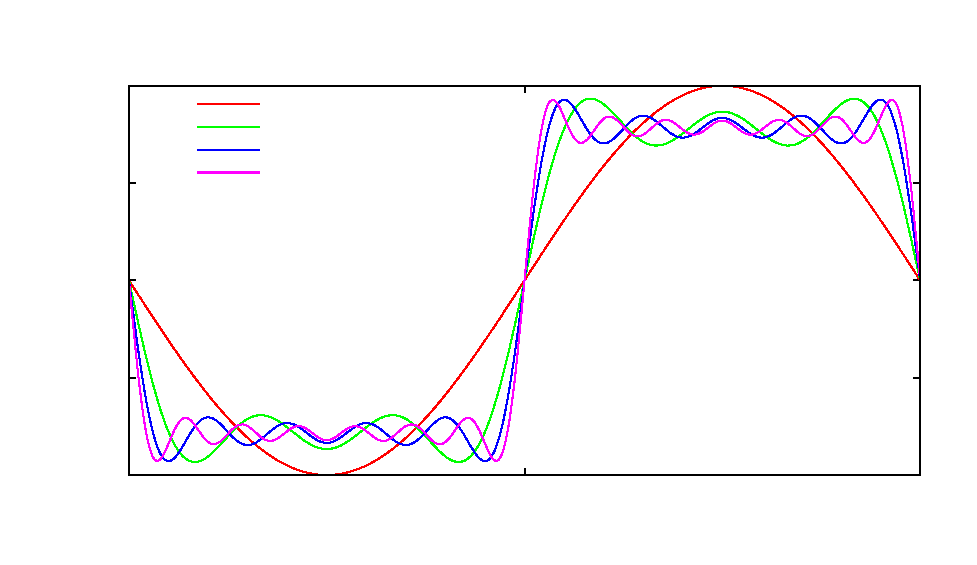
\includegraphics{Content/Intro/DummySection/Fouriersynthese/FourierOut}}%
    \gplfronttext
  \end{picture}%
\endgroup

	\caption{Eine Fouriersynthese}
	\label{fig:testfig}
\end{figure}

\bigskip
Und die dazu Passende Formel: \SeeEq{eq:fourier}
\index{Fouriersynthese}

\begin{equation}
	\sum_{i=0}^{n} \frac{1}{i \cdot 2 + 1} \cdot
	\sin \left( x \cdot \left( i \cdot 2 + 1 \right) \right)
	\label{eq:fourier}
\end{equation}

\clearpage
Und nun C++ Code: \SeeS{code:example}

\begin{c++}{Ein Stück Code}{code:example}
int main(int argc, char *argv[]) {
	int fd;
	int chars_sent;
	char buf[MAXBUF];

	if (argc < 3) {
		cerr << "argument missing, IP address an text needed, exiting..."<< endl;
		return 1;
	}

	/*
	 * multyrow comment
	 */

	// IP and Port
	sockaddr_in name;
	bzero(&name, sizeof(name));
	name.sin_family = AF_INET;
	inet_aton(argv[1], &(name.sin_addr));
	name.sin_port = htons(MYPORT);

	// connect to server
	DEBUG("try connect");
	if (connect(fd, (struct sockaddr *) &name, sizeof(name)) < 0) {
		PANIC("CONNECT");
	}
	// Transfer
	sprintf(buf, "%s:%s", argv[1], argv[2]);
	chars_sent = send(fd, buf, strlen(buf), 0);
	DEBUG("n=" << chars_sent << " Bytes sent");
	DEBUG("message length: " << strlen(buf));
	if (chars_sent < 0) {
		PANIC("SEND");
	}

	// close socket
	DEBUG("close socket");
	close(fd);

	return 0;
}
\end{c++}

Ein \index{Dummytext}Dummytext mit einer \ac{DUM} die öfter benutzt wird \ac{DUM}

\begin{longtable}{|c|m{12cm}|}
	\hline 
	Nummer & Anforderung \\
	\hline
	\EmptyRow 
	\hline \endhead
		\Textlabel{FA 1.1}{text:1} &
			Anforderung 1 \\
	\hline \Grayrow 
		\Textlabel{FA 1.2}{text:2} & 
			Anforderung 2\\ 
	\hline
	\CaptionLongtable{Funktionale Anforderungen an das Planungstool}
	\label{tab:FunctionalRequirements}
\end{longtable}

so kann darauf referenziert werden: \ref{text:1} \ref{text:2}
